% Contribution chapter no. 1 (TOP20 pick 1, id Z-BAO-P1) -- English translation of chapters/c01.tex
% Sources: papers/certified_bao/ (certified_bao.tex, publication_meta.json),
% results/certified_numerics/P1_bao/ (verification.md, bounds_Fit.json), TOP20.json.
\chapter[Cosmic distances, machine-checked]{Cosmic distances with an error margin checked by a machine}
\reference{Published on 8 October 2026.\\ doi:10.5281/\\zenodo.23247730}

\section*{The idea in one picture}

\begin{analogie}
At the end of the day, a very fast cash register announces the total sales. A distrustful inspector does not take its
word for it: he goes back over every receipt, one by one, and redoes the additions with a pencil. If he lands on the
same total, we know the sum is right, however the register worked it out. Here, the register is a fast calculation
program; the inspector with the pencil is the judge of a proof checker.

\emph{Where the picture stops:} the inspector checks the addition, not the prices. In the same way, the machine
certifies the calculation, not the model of the universe it was handed.
\end{analogie}

\section*{What was done}

To measure immense distances, astronomers use a ``standard ruler'' left behind in the young universe: baryon acoustic
oscillations (sound waves frozen into the distribution of matter). The large galaxy survey DESI published these
measurements in 2025 at seven ``redshifts'' $z$ (a way of saying ``how far away, and therefore how long ago''), from
$z=0.295$ to $z=2.33$. To compare a measurement with theory, you need a calculated distance, and that distance is an
area under a curve:
\[ \chi(z)=\int_0^z \frac{dx}{E(x)}, \qquad E(x)=\sqrt{\Omega_m(1+x)^3+1-\Omega_m}, \]
where $\Omega_m$ is the share of matter in the universe. An ordinary computer calculates this area by rounding at
every step: it gives a number very close to the true one, but with no written guarantee.

The trick used here is simple. The curve $1/E$ always goes down. If you cut the interval into small steps, the
rectangles placed ``under'' the curve have a total area smaller than the true one, and those that stick out above it
have a larger one (figure~\ref{fig:c01}a). The true distance is therefore caught between the two. A fast program,
which we do not trust, supplies for each of the 4,661 points of the subdivision two whole numbers, one a little below
and one a little above $1/E$. The judge then checks each pair with exact arithmetic on whole numbers, never
computing a single square root.

\begin{encadre}
\textbf{To do with a pencil.} How can you know, without a square root, that $1/\sqrt{2}$ lies between $0.70$ and
$0.71$? Square and multiply by $2$: $0.70^2\times2=0.98$, which is smaller than $1$, and
$0.71^2\times2=1.0082$, which is larger than $1$. So $0.70\le 1/\sqrt2\le 0.71$. This is exactly the kind of test the
machine repeats thousands of times, with twelve-digit whole numbers.

\textbf{The squeeze with a single step.} At the measurement point $z=0.295$, we have $1/E(0)=1$ and
$1/E(0.295)\approx0.8611$ (a value enclosed by the machine). With a single low rectangle and a single high
rectangle, $0.295\times0.8611\approx0.254\le\chi\le0.295\times1=0.295$. With 590 steps instead of one, the verified
enclosure becomes $0.2747074\le\chi\le0.2747769$.
\end{encadre}

The result: at the seven DESI redshifts, the distance is locked inside an interval whose relative width is between
$2.5$ and $2.8$ ten-thousandths, about $0.03$\,\% (figure~\ref{fig:c01}b). The calculation is done for a single
value, $\Omega_m=0.29743$, which comes from the fit made by the project itself (DESI publishes
$0.2975\pm0.0086$).

These enclosures were then used as a judge for other software. The project's Rust solver (a rewrite of CVODE, a
standard numerical tool) and the astropy library both fall inside them at all seven points. A deliberately sloppy
calculation (tolerance $10^{-2}$) falls outside at 3 of the 7 points. Finally, if $\Omega_m$ is increased by 1\,\%,
the new enclosures no longer overlap the old ones: the method can tell apart a 1\,\% change.

\begin{figure}[htbp]
\centering
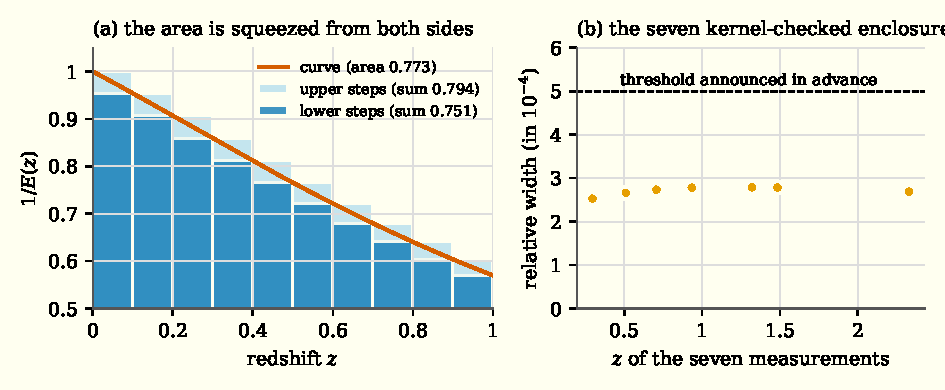
\includegraphics[width=\linewidth]{figures/c01_encadrement}
\caption{(a) The squeeze principle, drawn with 10 steps so that they can be seen (the real calculation uses 2,000 per
unit of $z$). (b) Relative width of the seven verified enclosures, read from the exact fractions in the theorems.}
\label{fig:c01}
\end{figure}

\section*{How we made sure it is not wrong}

\niveau{As} \emph{The judge looked, without a replay.} The judge here is Lean, a program that checks every logical
step of a proof; its core, the ``kernel'', verified the tables of whole numbers one by one, without the shortcut
that would trust the compiler. The 55 theorems use only the three basic assumptions accepted everywhere. However,
these files are not part of the full replay by a second checking program carried out on 26 October: hence the
label ``without a replay''.

Five hypotheses had been written down \emph{before} computing. Four were confirmed; the fifth (an enclosure of the
goodness of fit) was not attempted. Tests designed to fail did fail: a falsified table of integers (one bound lowered
by a million units) was rejected by the kernel; a fake ``proof'' left blank and a hidden axiom were both flagged by
the audit. A textbook case whose answer is known exactly (a universe made only of matter) falls properly inside its
enclosure.

An AI agent independent of the one that produced the work recompiled everything, added its own traps (which were
rejected), recomputed every distance with 50 exact digits, and gave a favourable opinion together with corrections to
the scope of the claims. Like this whole book, this work was produced by AI agents under the author's direction and
audited by other AI agents: no human specialist has reviewed it. The solver values, for their part, remain ordinary
calculations \niveau{X}.

\section*{What this does not say}

\begin{limite}
\begin{itemize}
\item A single value of $\Omega_m$, the project's own, and nothing guarantees that it is the best fit.
\item The model is imposed: a flat universe, without radiation. The machine does not say whether this model is the
right one.
\item The step to the quantities published by DESI and the comparison with their measurements are done outside Lean.
\item This is not a new measurement of the universe: it is a verified reference calculation.
\item The solver test is only as fine as the enclosure ($10^{-4}$): a calculation with tolerance $10^{-3}$ passes too.
\end{itemize}
\end{limite}

\section*{Going further}

The same method, certificates in whole numbers re-read by the kernel, was reused two days later for the whole
likelihood of the data (next chapter). Paper and files: doi:10.5281/zenodo.23247730.
